\chapter{Servlets}

\fcolorbox{black}[HTML]{E9F0E9}{\parbox{\textwidth}{%
\noindent \textbf{Learning goals}\\
The junior-colleague
\begin{enumerate}[nolistsep]
\item can explain what a Servlet is
\item can explain how Spring Boot uses Servlet technology (DispatcherServlet!)
\item can explain and use the lifecycle moments of a Servlet
\item can explain the usage of @WebServlet, @WebFilter and @WebListener
\item can explain the usage of HttpSession
\item can create an HTTPServlet to handle requests
\item can use cookies and HTTPSession in a web application
\item can use WebClient to send a simple HTTP request 
\item can implement a @WebFilter
\item can implement a @WebListener
\item can explain the Model-View-Controller design pattern
\item can explain the role of DispatcherServlet in Spring
\item can consume Rest services with WebClient
\item can implement a simple view with Thymeleaf
\end{enumerate}
}}

\fcolorbox{black}[HTML]{ADD8E6}{\parbox{\textwidth}{%
\noindent \textbf{Source for this chapter:}\\
\url{https://github.com/custersnele/servlet_technology.git}
}}

\section{What is a Servlet}

Relatively few applications still use Servlets directly,  but they're still the underlying technology behind the vast majority of Java and JVM web frameworks.
A servlet’s job is to take a client’s request and send back a response.
For example, we can use a Servlet to collect input from a user through an HTML form, query records from a database, and create web pages dynamically.
Servlets are under the control of another Java application called a Servlet Container. When an application running in a web server receives a request, the server hands the request to the Servlet Container – which in turn passes it to the target Servlet.
Java servlets typically run on the HTTP protocol. 

When using Spring Boot, the @ServletComponentScan annotation automatically registers the Servlet components for embedded web servers. This annotation supports the following Servlet 3.0 annotations:
\begin{itemize}
\item @WebServlet annotation
\item @WebFilter annotation
\item @WebListener annotation
\end{itemize}

\begin{lstlisting}
package be.pxl.paj.servlets;

import org.springframework.boot.SpringApplication;
import org.springframework.boot.autoconfigure.SpringBootApplication;
import org.springframework.boot.web.servlet.ServletComponentScan;

@SpringBootApplication
@ServletComponentScan
public class ServletDemoApplication {

	public static void main(String[] args) {
		SpringApplication.run(ServletDemoApplication.class, args);
	}
}
\end{lstlisting}

\section{Servlet class hierarchy}

The Servlet interface is the root interface of the servlet class hierarchy. All Servlets need to either directly or indirectly implement the Servlet interface. 

The Servlet interface of the jakarta.servlet package defines the methods that the Servlet container calls to manage the servlet life cycle. 

The GenericServlet class of the Servlet API implements the Servlet interface.

To develop a servlet that communicates using HTTP, we need to extend the HttpServlet class.

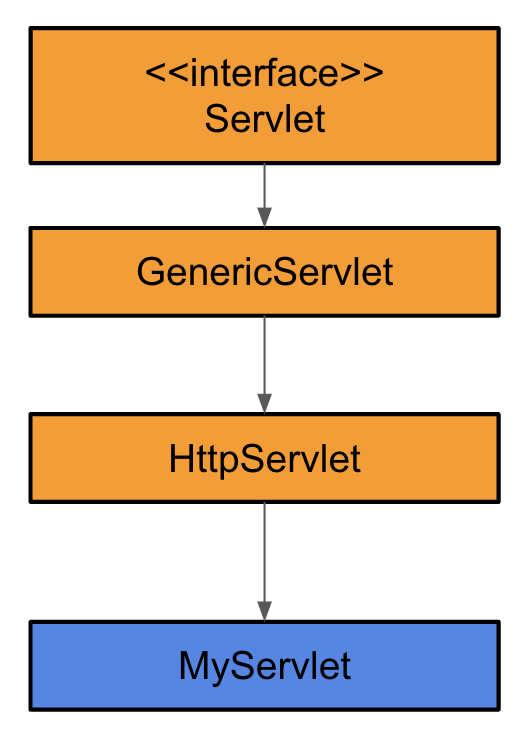
\includegraphics{./images/chapter8/servlet_hierarchy}


\section{Lifecycle of a servlet}

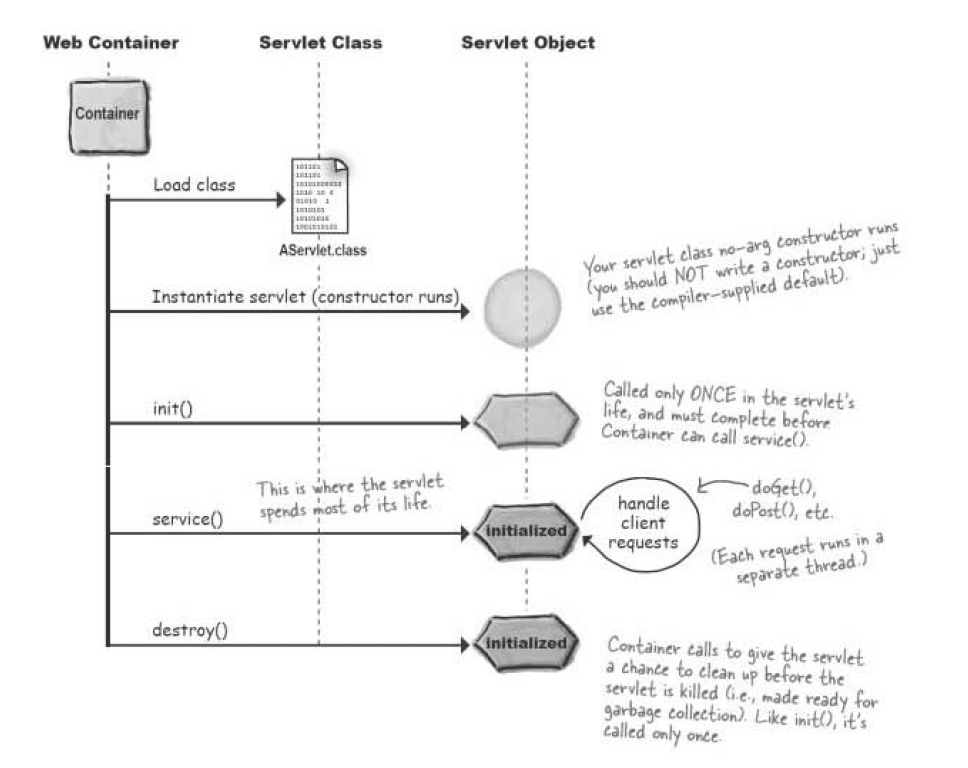
\includegraphics[width=\textwidth]{./images/chapter8/servlet_lifecycle}

The Servlet life cycle mainly goes through three stages:\cite{servlet_lifecycle}

\begin{itemize}
\item \textbf{Loading and initializing a Servlet.} After the Servlet is instantiated successfully, the Servlet container initializes the instantiated Servlet object. The container initializes the Servlet object by invoking the \textbf{init()} method. The jakarta.servlet.ServletConfig interface is implemented by a Servlet container to pass configuration information to a servlet, during initialization of a servlet.
\item \textbf{Request handling.} After initialization, the Servlet instance is ready to serve the client requests.  The Servlet's \textbf{service()} method is invoked to handle a client request. When multiple client requests come, the server will create multiple threads. Each client request corresponds to a thread that calls the Servlet's service() method.  That's the nice thing about Java, it's multithreaded and different threads (HTTP requests) can make use of the same instance. It would otherwise be too expensive to recreate, init() and destroy() them for every single request. If you encounter threadsafety issues when using servlets, then it is your fault, not Java's nor Servlet's fault.
\item \textbf{Destroying the Servlet.} When a Servlet container decides to destroy the Servlet,  all currently running threads can complete their jobs and next, the Servlet container calls the destroy() method on the Servlet instance.
\end{itemize}

\subsection{Example 1}

\begin{lstlisting}[language=java, frame=single]
package be.pxl.paj.servlets;

import jakarta.servlet.annotation.WebServlet;
import jakarta.servlet.http.HttpServlet;
import jakarta.servlet.http.HttpServletRequest;
import jakarta.servlet.http.HttpServletResponse;
import java.io.IOException;
import java.io.PrintWriter;
import java.time.LocalDateTime;
import java.time.format.DateTimeFormatter;
import java.util.Locale;

@WebServlet(value="/DateTimeServlet")
public class DateTimeServlet extends HttpServlet {

	private static final DateTimeFormatter FORMATTER_EN = DateTimeFormatter.ofPattern("EEEE dd/MM/yyyy HH:mm:ss", Locale.ENGLISH);
	private static final DateTimeFormatter FORMATTER_NL = DateTimeFormatter.ofPattern("EEEE dd/MM/yyyy HH:mm:ss", new Locale("nl"));

	@Override
	protected void doGet(HttpServletRequest req, HttpServletResponse resp) throws IOException {
		PrintWriter writer = resp.getWriter();
		String language = req.getParameter("lang");
		LocalDateTime dateTime = LocalDateTime.now();
		String dateAsText = "nl".equals(language) ? 
		         FORMATTER_NL.format(dateTime) : FORMATTER_EN.format(dateTime);
		writer.println("<html>" +
				"<body>" +
				"<h1 style=\"text-align:center\">" + dateAsText + "</h1></body>" +
				"</html>");
	}
}
\end{lstlisting}


\subsection{Example 2}


\begin{lstlisting}[frame=single, language=html]
<!DOCTYPE html>
<html lang="en">
<head>
	<meta charset="UTF-8">
	<title>Beer selection</title>
</head>
<body>
<h1>Beer Selection</h1>
<form method="POST" action="/SelectBeer.do">
	<p>Select beer characteristics:</p>
	<label for="color">Color:</label>
	<select id="color" name="color" size="1">
		<option value="light">Light</option>
		<option value="amber">Amber</option>
		<option value="brown">Brown</option>
		<option value="dark">Dark</option>
	</select>
	<br/>
	<br/>
	<input type="submit" />
</form>
</body>
</html>
\end{lstlisting}

\begin{lstlisting}[frame=single, language=java]
package be.pxl.paj.servlets;

import be.pxl.paj.servlets.service.BeerExpert;
import org.springframework.beans.factory.annotation.Autowired;

import jakarta.servlet.ServletException;
import jakarta.servlet.annotation.WebServlet;
import jakarta.servlet.http.HttpServlet;
import jakarta.servlet.http.HttpServletRequest;
import jakarta.servlet.http.HttpServletResponse;
import java.io.IOException;
import java.io.PrintWriter;
import java.util.List;

@WebServlet(value = "/SelectBeer.do")
public class SelectBeerServlet extends HttpServlet {

	private final BeerExpert beerExpert;

	@Autowired
	public SelectBeerServlet(BeerExpert beerExpert) {
		this.beerExpert = beerExpert;
	}

	@Override
	protected void doPost(HttpServletRequest req, HttpServletResponse resp) throws ServletException, IOException {
		String color = req.getParameter("color");

		List<String> result = beerExpert.getBrands(color);
		PrintWriter writer = resp.getWriter();

		writer.println("<html>" +
				"<body>" +
				"<h1 style=\"text-align:center\">Try these beers:</h1><p>" +
				String.join(", ", result) +
				"</p></body>" +
				"</html>");
	}
}
\end{lstlisting}

\begin{lstlisting}[frame=single, language=java]
package be.pxl.paj.servlets.service;

import org.springframework.stereotype.Service;

import java.util.ArrayList;
import java.util.List;

@Service
public class BeerExpert {

	public List<String> getBrands(String color) {
		List<String> brands = new ArrayList<>();
		if (color.equals("amber")) {
			brands.add("Jack Amber");
			brands.add("Red Moose");
		} else {
			brands.add("Jail Pale Ale");
			brands.add("Gout Stout");
		}
		return brands;
	}
}
\end{lstlisting}


\section{Session tracking}

Session management is a way to maintain state of an user. 

HTTP protocol is a stateless so we need to maintain state using session management techniques. Each time user requests to the server, server treats the request as the new request. 

There are several techniques for session management:

\begin{itemize}
\item Cookies
\item Hidden Form Field
\item URL Rewriting
\item HttpSession
\end{itemize}

In this course we will provide examples for using cookies and HttpSession.

\subsection{Cookies}

The method getCookies() in HttpServletRequest returns an array containing all of the Cookie objects the client sent with this request. 

\begin{lstlisting}[language=java, frame=single]
package be.pxl.paj.servlets;

import jakarta.servlet.annotation.WebServlet;
import jakarta.servlet.http.Cookie;
import jakarta.servlet.http.HttpServlet;
import jakarta.servlet.http.HttpServletRequest;
import jakarta.servlet.http.HttpServletResponse;
import java.io.IOException;
import java.io.PrintWriter;

@WebServlet(name = "Cookies", value = "/Cookies")
public class UsingCookies extends HttpServlet {

	public void doGet(HttpServletRequest request, HttpServletResponse response)
			throws IOException {
		response.setContentType("text/html");
		PrintWriter out = response.getWriter();

		out.println("<HTML>");
		out.println("<HEAD>");
		out.println("<TITLE>");
		out.println("A Web Page");
		out.println("</TITLE>");
		out.println("</HEAD>");
		out.println("<BODY");

		Cookie[] cookies = request.getCookies();
		boolean foundCookie = false;

		for (int loopIndex = 0; loopIndex < cookies.length; loopIndex++) {
			Cookie cookie1 = cookies[loopIndex];
			if (cookie1.getName().equals("color")) {
				out.println("bgcolor = " + cookie1.getValue());
				foundCookie = true;
			}
		}

		if (!foundCookie) {
			Cookie cookie1 = new Cookie("color", "cyan");
			cookie1.setMaxAge(24 * 60 * 60);
			response.addCookie(cookie1);
		}

		out.println(">");
		out.println("<H1>Setting and Reading Cookies</H1>");
		out.println("This page will set its background color using a cookie when reloaded.");
		out.println("</BODY>");
		out.println("</HTML>");
	}
}
\end{lstlisting}

\subsection{HttpSession}

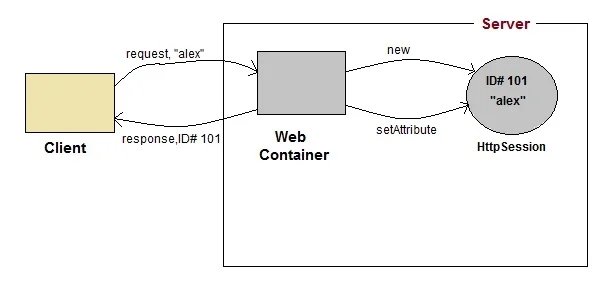
\includegraphics[width=\textwidth]{./images/chapter8/httpsession}

HTTP sessions are identified by a unique session ID.  A session ID is a pseudo-random number generated at the runtime. 

On client's first request, the Web Container generates a unique session ID and gives it back to the client encapsulated in the response. 
The client sends back the session ID with each request. This way the web container can identify where the request is coming from.
The Web Container uses this ID, finds the matching session with the ID and associates the session with the request.

Session hijacking is a known attack for HTTP sessions and can be prevented if all the requests going over the network are enforced to be over a secure connection (meaning, HTTPS).

Below is the click\_the\_button.html file.  There are several directories where you can store static html pages. In our demo we've chosen to create a folder named `static' in the application's resources folder.
\begin{lstlisting}[language=html]
<!DOCTYPE html>
<html lang="en">
<head>
	<meta charset="UTF-8">
	<title>Click the Button!</title>
</head>
<body>
<h1>Click the button!</h1>
<form action="/ButtonClicked" method="POST">
	<input type="submit" value="Click me!">
</form>
</body>
</html>
\end{lstlisting}

\begin{lstlisting}[language=java, frame=single]
package be.pxl.paj.servlets;

import java.io.IOException;

import jakarta.servlet.ServletException;
import jakarta.servlet.annotation.WebServlet;
import jakarta.servlet.http.HttpServlet;
import jakarta.servlet.http.HttpServletRequest;
import jakarta.servlet.http.HttpServletResponse;
import jakarta.servlet.http.HttpSession;

@WebServlet(name = "/ButtonClicked", value="/ButtonClicked")
public class ButtonClickedServlet extends HttpServlet {

	@Override
	public void doPost(HttpServletRequest request, 
	                                 HttpServletResponse response) throws IOException, ServletException {

		int clickCount = 0;

		//get the session, which contains user-specific data
		HttpSession session = request.getSession();

		if(session.getAttribute("clickCount") != null){
			//we've already stored the clickCount in a previous request, so get it
			clickCount = (int) session.getAttribute("clickCount");
		}

		clickCount++;

		//store the new clickCount in the session
		session.setAttribute("clickCount", clickCount);

		//output the clickCount for this user
		response.getOutputStream().println("<h1>You clicked the button " + clickCount + " times.</h1>");
		response.getOutputStream().println("<p>Click <a href=\"/click_the_button.html\">here</a> to go back to the button.</p>");
	}
}
\end{lstlisting}


\section{Spring DispatcherServlet}


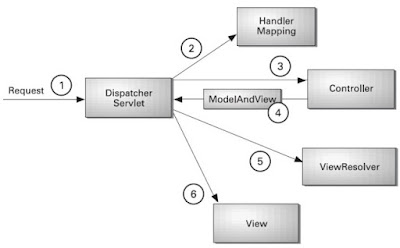
\includegraphics{./images/chapter8/spring_mvc}

The Spring web framework is built around the MVC (Model-View-Controller) pattern.
In Spring Web MVC,  all the incoming request are intercepted by the DispatcherServlet that works as a front controller. The DispatcherServlet forwards the request to the controller reponsible for handling the request, i.e. the controller that matches the requested URL.   The controller returns a response, besides REST responses, objects of ModelAndView can be returned as well.  If a ModelAndView response is returned, the  DispatcherServlet invokes the specified view component.

The MVC pattern was first introduced in 1979 by computer scientist Trygve Mikkjel Heyerdahl Reenskaug. He wanted to come up with a solution on how to break up a complex user application into smaller manageable components.

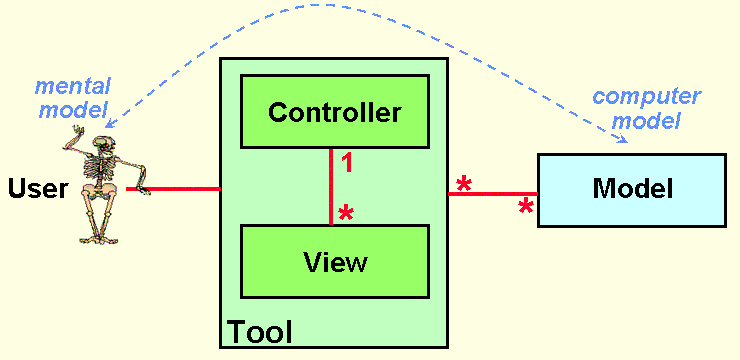
\includegraphics[width=\textwidth]{./images/chapter8/original_mvc}

This is a basic breakdown of the MVC pattern:

\begin{itemize}
\item Model - A model contains the data of the application.  
\item Controller - A controller interprets user input and transform it into a model that is represented to the user by the view.  The controller is responsible for processing user requests and building an appropriate model and passes it to the view for rendering. Here, the @Controller annotation is used to mark the class as the controller.
\item View - A view represents the provided information in a particular format.  Spring also supports view technologies such as Apache Velocity,  Thymeleaf and FreeMarker.
\end{itemize}

In Spring Web MVC,  we have this extra component, the DispatcherServlet class, which works as the front controller. It is responsible to manage the flow of the Spring MVC application.


\subsection{Views}

This section shows how Thymeleaf can be used as an template engine by Spring Boot.

First we add the dependency.

\begin{lstlisting}[frame=single]
<dependency>
	<groupId>org.springframework.boot</groupId>
	<artifactId>spring-boot-starter-thymeleaf</artifactId>
</dependency>
\end{lstlisting}

By default, Spring Boot looks for  templates in the directory src/main/resources/templates. 

We have two templates,  on for submitting a country name and a second for displaying the universities of the chosen country. 

\begin{lstlisting}[language=html, frame=single]
<!DOCTYPE html>
<html lang="en">
<head>
	<meta charset="UTF-8">
	<title>Search universities</title>
</head>
<body>
<form th:action="@{/universities}">
	<div>
		<label>Country:</label>
		<input type="text" th:name="country" />
	</div>
	<input type="submit"/>
</form>
</body>
</html>
\end{lstlisting}

\begin{lstlisting}[language=html, frame=single]
<!DOCTYPE html>
<html lang="en">
<head>
	<meta charset="UTF-8">
	<title>Title</title>
</head>
<body>
<div th:each="university : ${universities}">
	<a th:href="${university.webPages.get(0)}"><p th:text="${university.name}"></a>
</div>
</body>
</html>
\end{lstlisting}

Let's have a look at the controller.

\begin{lstlisting}[language=java, frame=single]
package be.pxl.paj.servlets.rest;

import be.pxl.paj.servlets.domain.University;
import org.springframework.stereotype.Controller;
import org.springframework.ui.Model;
import org.springframework.web.bind.annotation.GetMapping;
import org.springframework.web.bind.annotation.RequestMapping;
import org.springframework.web.bind.annotation.RequestParam;
import org.springframework.web.reactive.function.client.WebClient;

@Controller
public class UniversityController {

	private final WebClient webClient = WebClient.create("http://universities.hipolabs.com");

	@GetMapping("/country_selection")
	public String countrySelection() {
		return "country_selection";
	}

	@RequestMapping("/universities")
	public String addUser(@RequestParam(value = "country") String country, Model model) {
		WebClient.ResponseSpec response = webClient.get()
				.uri(String.format("search?country=%s", country))
				.retrieve();
		University[] universities = response.bodyToMono(University[].class).block();
		model.addAttribute("universities", universities);
		return "universities";
	}
}

\end{lstlisting}

The University class is a POJO-class.

\begin{lstlisting}[language=java, frame=single]
package be.pxl.paj.servlets.domain;

import com.fasterxml.jackson.annotation.JsonProperty;

import java.util.List;

public class University {
	private String name;
	@JsonProperty("web_pages")
	private List<String> webPages;

	public String getName() {
		return name;
	}

	public List<String> getWebPages() {
		return webPages;
	}
}
\end{lstlisting}


\section{@WebFilter}

Filters let you intercept the request.  And if you can intercept the request,
you can also control the response.  And, the servlet  never
knows that someone stepped in between the client request and the servlet container’s invocation 
of the servlet’s service() method.  Therefore,  if you choose to write and configure a filter, you're able to affect all of your servlets.  For example, if you want to add
user request tracking to every servlet in your application or manipulate the output
from every servlet? No problem.  Just write a filter and you don’t even have to touch the servlets.

\begin{lstlisting}[language=java, frame=single]
package be.pxl.paj.servlets;


import org.apache.logging.log4j.LogManager;
import org.apache.logging.log4j.Logger;

import jakarta.servlet.Filter;
import jakarta.servlet.FilterChain;
import jakarta.servlet.ServletException;
import jakarta.servlet.ServletRequest;
import jakarta.servlet.ServletResponse;
import jakarta.servlet.annotation.WebFilter;
import jakarta.servlet.http.HttpServletRequest;
import jakarta.servlet.http.HttpServletResponse;
import java.io.IOException;
import java.util.Collections;

@WebFilter(urlPatterns = { "/SelectBeer.do" })
public class HeaderLogFilter implements Filter {

	private static final Logger LOGGER = LogManager.getLogger(HeaderLogFilter.class);

	@Override
	public void doFilter(ServletRequest request, ServletResponse response,
	                     FilterChain chain) throws IOException, ServletException {
		HttpServletRequest req = (HttpServletRequest) request;
		HttpServletResponse rep = (HttpServletResponse) response;

		LOGGER.info("----- Request ---------");
		Collections.list(req.getHeaderNames()).forEach(n -> LOGGER.info(n + ": " + req.getHeader(n)));

		chain.doFilter(request, response);

		LOGGER.info("----- response ---------");

		rep.getHeaderNames().forEach(n -> LOGGER.info(n + ": " + rep.getHeader(n)));

		LOGGER.info("response status: " + rep.getStatus());
	}
}
\end{lstlisting}


\section{@WebListener}

@WebListener annotation is used to define a servlet listener component in a web application.

Many listeners are defined for events involving life cycles of ServletContext, HttpSession and ServletRequest.  Following listeners are supported for @WebListener:

\begin{itemize}
\item jakarta.servlet.ServletContextListener
\item jakarta.servlet.ServletContextAttributeListener
\item jakarta.servlet.ServletRequestListener
\item jakarta.servlet.ServletRequestAttributeListener
\item jakarta.servlet.http.HttpSessionListener
\item jakarta.servlet.http.HttpSessionAttributeListener
\end{itemize}


\begin{lstlisting}[language=java, frame=single]
package be.pxl.paj.servlets;

import jakarta.servlet.ServletContextEvent;
import jakarta.servlet.ServletContextListener;
import jakarta.servlet.annotation.WebListener;

@WebListener
public class ExampleContextListener implements ServletContextListener {

	@Override
	public void contextInitialized(ServletContextEvent servletContextEvent) {
		System.out.println("ServletDemo starting up!");
	}

	@Override
	public void contextDestroyed(ServletContextEvent servletContextEvent) {
		System.out.println("ServletDemo shutting down!");
	}
}
\end{lstlisting}

\section{Exercises}

\begin{oefening}
The html-page phonebook\_add.html is provided. Create a Servlet to handle the form’s POST request. The data is saved to a (in-memory) database. Make sure the phonenumber is unique.  Create a Servlet to display all the entries in the phonebook. 
\end{oefening}

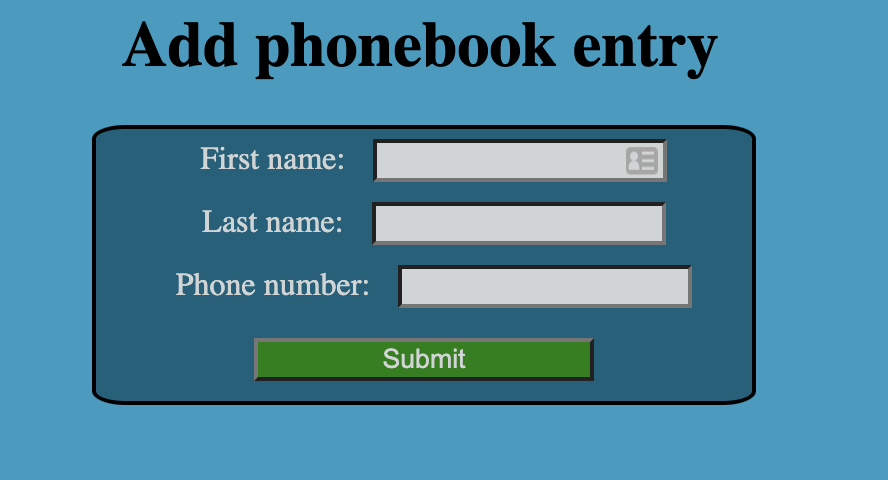
\includegraphics{./images/chapter8/add_phonebook_entry}
